\documentclass[1p]{elsarticle_modified}
%\bibliographystyle{elsarticle-num}

%\usepackage[colorlinks]{hyperref}
%\usepackage{abbrmath_seonhwa} %\Abb, \Ascr, \Acal ,\Abf, \Afrak
\usepackage{amsfonts}
\usepackage{amssymb}
\usepackage{amsmath}
\usepackage{amsthm}
\usepackage{scalefnt}
\usepackage{amsbsy}
\usepackage{kotex}
\usepackage{caption}
\usepackage{subfig}
\usepackage{color}
\usepackage{graphicx}
\usepackage{xcolor} %% white, black, red, green, blue, cyan, magenta, yellow
\usepackage{float}
\usepackage{setspace}
\usepackage{hyperref}

\usepackage{tikz}
\usetikzlibrary{arrows}

\usepackage{multirow}
\usepackage{array} % fixed length table
\usepackage{hhline}

%%%%%%%%%%%%%%%%%%%%%
\makeatletter
\renewcommand*\env@matrix[1][\arraystretch]{%
	\edef\arraystretch{#1}%
	\hskip -\arraycolsep
	\let\@ifnextchar\new@ifnextchar
	\array{*\c@MaxMatrixCols c}}
\makeatother %https://tex.stackexchange.com/questions/14071/how-can-i-increase-the-line-spacing-in-a-matrix
%%%%%%%%%%%%%%%

\usepackage[normalem]{ulem}

\newcommand{\msout}[1]{\ifmmode\text{\sout{\ensuremath{#1}}}\else\sout{#1}\fi}
%SOURCE: \msout is \stkout macro in https://tex.stackexchange.com/questions/20609/strikeout-in-math-mode

\newcommand{\cancel}[1]{
	\ifmmode
	{\color{red}\msout{#1}}
	\else
	{\color{red}\sout{#1}}
	\fi
}

\newcommand{\add}[1]{
	{\color{blue}\uwave{#1}}
}

\newcommand{\replace}[2]{
	\ifmmode
	{\color{red}\msout{#1}}{\color{blue}\uwave{#2}}
	\else
	{\color{red}\sout{#1}}{\color{blue}\uwave{#2}}
	\fi
}

\newcommand{\Sol}{\mathcal{S}} %segment
\newcommand{\D}{D} %diagram
\newcommand{\A}{\mathcal{A}} %arc


%%%%%%%%%%%%%%%%%%%%%%%%%%%%%5 test

\def\sl{\operatorname{\textup{SL}}(2,\Cbb)}
\def\psl{\operatorname{\textup{PSL}}(2,\Cbb)}
\def\quan{\mkern 1mu \triangleright \mkern 1mu}

\theoremstyle{definition}
\newtheorem{thm}{Theorem}[section]
\newtheorem{prop}[thm]{Proposition}
\newtheorem{lem}[thm]{Lemma}
\newtheorem{ques}[thm]{Question}
\newtheorem{cor}[thm]{Corollary}
\newtheorem{defn}[thm]{Definition}
\newtheorem{exam}[thm]{Example}
\newtheorem{rmk}[thm]{Remark}
\newtheorem{alg}[thm]{Algorithm}

\newcommand{\I}{\sqrt{-1}}
\begin{document}

%\begin{frontmatter}
%
%\title{Boundary parabolic representations of knots up to 8 crossings}
%
%%% Group authors per affiliation:
%\author{Yunhi Cho} 
%\address{Department of Mathematics, University of Seoul, Seoul, Korea}
%\ead{yhcho@uos.ac.kr}
%
%
%\author{Seonhwa Kim} %\fnref{s_kim}}
%\address{Center for Geometry and Physics, Institute for Basic Science, Pohang, 37673, Korea}
%\ead{ryeona17@ibs.re.kr}
%
%\author{Hyuk Kim}
%\address{Department of Mathematical Sciences, Seoul National University, Seoul 08826, Korea}
%\ead{hyukkim@snu.ac.kr}
%
%\author{Seokbeom Yoon}
%\address{Department of Mathematical Sciences, Seoul National University, Seoul, 08826,  Korea}
%\ead{sbyoon15@snu.ac.kr}
%
%\begin{abstract}
%We find all boundary parabolic representation of knots up to 8 crossings.
%
%\end{abstract}
%\begin{keyword}
%    \MSC[2010] 57M25 
%\end{keyword}
%
%\end{frontmatter}

%\linenumbers
%\tableofcontents
%
\newcommand\colored[1]{\textcolor{white}{\rule[-0.35ex]{0.8em}{1.4ex}}\kern-0.8em\color{red} #1}%
%\newcommand\colored[1]{\textcolor{white}{ #1}\kern-2.17ex	\textcolor{white}{ #1}\kern-1.81ex	\textcolor{white}{ #1}\kern-2.15ex\color{red}#1	}

{\Large $\underline{12n_{0135}~(K12n_{0135})}$}

\setlength{\tabcolsep}{10pt}
\renewcommand{\arraystretch}{1.6}
\vspace{1cm}\begin{tabular}{m{100pt}>{\centering\arraybackslash}m{274pt}}
\multirow{5}{120pt}{
	\centering
	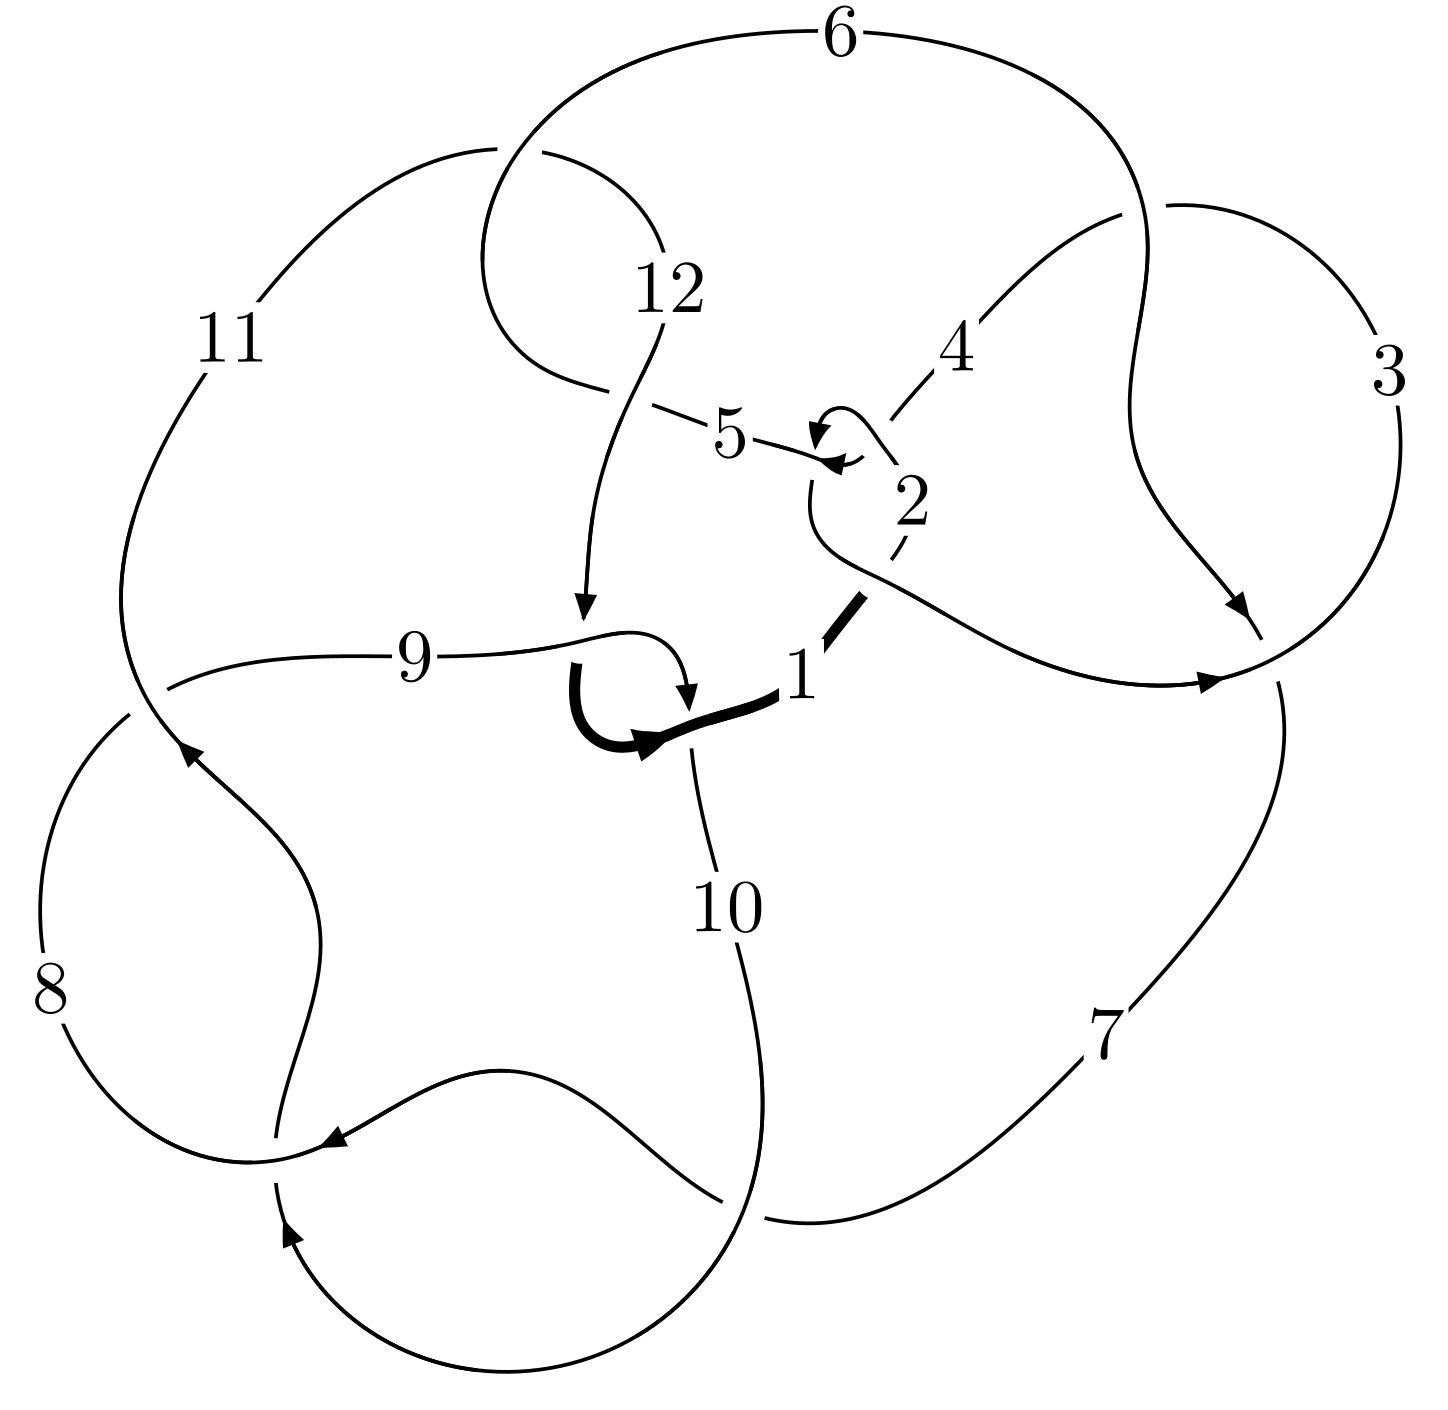
\includegraphics[width=112pt]{../../../GIT/diagram.site/Diagrams/png/2224_12n_0135.png}\\
\ \ \ A knot diagram\footnotemark}&
\allowdisplaybreaks
\textbf{Linearized knot diagam} \\
\cline{2-2}
 &
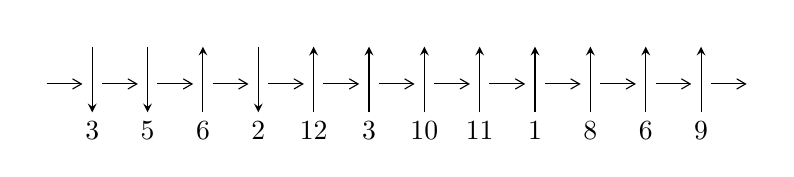
\begin{tikzpicture}[x=20pt, y=17pt]
	% nodes
	\node (C0) at (0, 0) {};
	\node (C1) at (1, 0) {};
	\node (C1U) at (1, +1) {};
	\node (C1D) at (1, -1) {3};

	\node (C2) at (2, 0) {};
	\node (C2U) at (2, +1) {};
	\node (C2D) at (2, -1) {5};

	\node (C3) at (3, 0) {};
	\node (C3U) at (3, +1) {};
	\node (C3D) at (3, -1) {6};

	\node (C4) at (4, 0) {};
	\node (C4U) at (4, +1) {};
	\node (C4D) at (4, -1) {2};

	\node (C5) at (5, 0) {};
	\node (C5U) at (5, +1) {};
	\node (C5D) at (5, -1) {12};

	\node (C6) at (6, 0) {};
	\node (C6U) at (6, +1) {};
	\node (C6D) at (6, -1) {3};

	\node (C7) at (7, 0) {};
	\node (C7U) at (7, +1) {};
	\node (C7D) at (7, -1) {10};

	\node (C8) at (8, 0) {};
	\node (C8U) at (8, +1) {};
	\node (C8D) at (8, -1) {11};

	\node (C9) at (9, 0) {};
	\node (C9U) at (9, +1) {};
	\node (C9D) at (9, -1) {1};

	\node (C10) at (10, 0) {};
	\node (C10U) at (10, +1) {};
	\node (C10D) at (10, -1) {8};

	\node (C11) at (11, 0) {};
	\node (C11U) at (11, +1) {};
	\node (C11D) at (11, -1) {6};

	\node (C12) at (12, 0) {};
	\node (C12U) at (12, +1) {};
	\node (C12D) at (12, -1) {9};
	\node (C13) at (13, 0) {};

	% arrows
	\draw[->,>={angle 60}]
	(C0) edge (C1) (C1) edge (C2) (C2) edge (C3) (C3) edge (C4) (C4) edge (C5) (C5) edge (C6) (C6) edge (C7) (C7) edge (C8) (C8) edge (C9) (C9) edge (C10) (C10) edge (C11) (C11) edge (C12) (C12) edge (C13) ;	\draw[->,>=stealth]
	(C1U) edge (C1D) (C2U) edge (C2D) (C3D) edge (C3U) (C4U) edge (C4D) (C5D) edge (C5U) (C6D) edge (C6U) (C7D) edge (C7U) (C8D) edge (C8U) (C9D) edge (C9U) (C10D) edge (C10U) (C11D) edge (C11U) (C12D) edge (C12U) ;
	\end{tikzpicture} \\
\hhline{~~} \\& 
\textbf{Solving Sequence} \\ \cline{2-2} 
 &
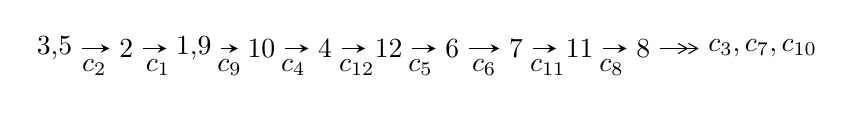
\begin{tikzpicture}[x=23pt, y=7pt]
	% node
	\node (A0) at (-1/8, 0) {3,5};
	\node (A1) at (1, 0) {2};
	\node (A2) at (33/16, 0) {1,9};
	\node (A3) at (25/8, 0) {10};
	\node (A4) at (33/8, 0) {4};
	\node (A5) at (41/8, 0) {12};
	\node (A6) at (49/8, 0) {6};
	\node (A7) at (57/8, 0) {7};
	\node (A8) at (65/8, 0) {11};
	\node (A9) at (73/8, 0) {8};
	\node (C1) at (1/2, -1) {$c_{2}$};
	\node (C2) at (3/2, -1) {$c_{1}$};
	\node (C3) at (21/8, -1) {$c_{9}$};
	\node (C4) at (29/8, -1) {$c_{4}$};
	\node (C5) at (37/8, -1) {$c_{12}$};
	\node (C6) at (45/8, -1) {$c_{5}$};
	\node (C7) at (53/8, -1) {$c_{6}$};
	\node (C8) at (61/8, -1) {$c_{11}$};
	\node (C9) at (69/8, -1) {$c_{8}$};
	\node (A10) at (11, 0) {$c_{3},c_{7},c_{10}$};

	% edge
	\draw[->,>=stealth]	
	(A0) edge (A1) (A1) edge (A2) (A2) edge (A3) (A3) edge (A4) (A4) edge (A5) (A5) edge (A6) (A6) edge (A7) (A7) edge (A8) (A8) edge (A9) ;
	\draw[->>,>={angle 60}]	
	(A9) edge (A10);
\end{tikzpicture} \\ 

\end{tabular} \\

\footnotetext{
The image of knot diagram is generated by the software ``\textbf{Draw programme}" developed by Andrew Bartholomew(\url{http://www.layer8.co.uk/maths/draw/index.htm\#Running-draw}), where we modified some parts for our purpose(\url{https://github.com/CATsTAILs/LinksPainter}).
}\phantom \\ \newline 
\centering \textbf{Ideals for irreducible components\footnotemark of $X_{\text{par}}$} 
 
\begin{align*}
I^u_{1}&=\langle 
7.50785\times10^{65} u^{51}+7.16783\times10^{66} u^{50}+\cdots+7.42713\times10^{65} b+1.96991\times10^{66},\\
\phantom{I^u_{1}}&\phantom{= \langle  }5.02177\times10^{66} u^{51}+4.81887\times10^{67} u^{50}+\cdots+1.48543\times10^{66} a+4.88267\times10^{67},\;u^{52}+10 u^{51}+\cdots+42 u+1\rangle \\
I^u_{2}&=\langle 
3 a^7- a^6-4 a^5+3 a^4+6 a^3-2 a^2+b-3 a+4,\;a^8- a^7- a^6+2 a^5+a^4-2 a^3+2 a-1,\;u-1\rangle \\
I^u_{3}&=\langle 
- u^4- u^3+u^2+b+2 u+1,\;u^5+u^4- u^3- u^2+a+u+1,\;u^6+u^5- u^4-2 u^3+u+1\rangle \\
\\
\end{align*}
\raggedright * 3 irreducible components of $\dim_{\mathbb{C}}=0$, with total 66 representations.\\
\footnotetext{All coefficients of polynomials are rational numbers. But the coefficients are sometimes approximated in decimal forms when there is not enough margin.}
\newpage
\renewcommand{\arraystretch}{1}
\centering \section*{I. $I^u_{1}= \langle 7.51\times10^{65} u^{51}+7.17\times10^{66} u^{50}+\cdots+7.43\times10^{65} b+1.97\times10^{66},\;5.02\times10^{66} u^{51}+4.82\times10^{67} u^{50}+\cdots+1.49\times10^{66} a+4.88\times10^{67},\;u^{52}+10 u^{51}+\cdots+42 u+1 \rangle$}
\flushleft \textbf{(i) Arc colorings}\\
\begin{tabular}{m{7pt} m{180pt} m{7pt} m{180pt} }
\flushright $a_{3}=$&$\begin{pmatrix}1\\0\end{pmatrix}$ \\
\flushright $a_{5}=$&$\begin{pmatrix}0\\u\end{pmatrix}$ \\
\flushright $a_{2}=$&$\begin{pmatrix}1\\- u^2\end{pmatrix}$ \\
\flushright $a_{1}=$&$\begin{pmatrix}- u^2+1\\- u^2\end{pmatrix}$ \\
\flushright $a_{9}=$&$\begin{pmatrix}-3.38070 u^{51}-32.4410 u^{50}+\cdots-334.790 u-32.8705\\-1.01087 u^{51}-9.65087 u^{50}+\cdots-83.4897 u-2.65231\end{pmatrix}$ \\
\flushright $a_{10}=$&$\begin{pmatrix}-4.55808 u^{51}-43.5756 u^{50}+\cdots-423.069 u-35.6566\\-0.649601 u^{51}-6.17332 u^{50}+\cdots-52.5054 u-1.87796\end{pmatrix}$ \\
\flushright $a_{4}=$&$\begin{pmatrix}u\\- u^3+u\end{pmatrix}$ \\
\flushright $a_{12}=$&$\begin{pmatrix}-0.0984110 u^{51}-0.192798 u^{50}+\cdots+107.102 u+18.1612\\-0.0523888 u^{51}-0.301105 u^{50}+\cdots+24.7289 u+0.984872\end{pmatrix}$ \\
\flushright $a_{6}=$&$\begin{pmatrix}1.75053 u^{51}+16.1107 u^{50}+\cdots+66.9644 u-4.72365\\0.445418 u^{51}+4.10330 u^{50}+\cdots+21.4257 u+0.355988\end{pmatrix}$ \\
\flushright $a_{7}=$&$\begin{pmatrix}2.19594 u^{51}+20.2140 u^{50}+\cdots+88.3901 u-4.36766\\0.445418 u^{51}+4.10330 u^{50}+\cdots+21.4257 u+0.355988\end{pmatrix}$ \\
\flushright $a_{11}=$&$\begin{pmatrix}-0.520552 u^{51}-4.34536 u^{50}+\cdots+41.7074 u+19.0709\\-0.0705558 u^{51}-0.589302 u^{50}+\cdots+8.55893 u+0.631584\end{pmatrix}$ \\
\flushright $a_{8}=$&$\begin{pmatrix}0.281350 u^{51}+1.78079 u^{50}+\cdots-103.579 u-19.6506\\-0.196558 u^{51}-1.93868 u^{50}+\cdots-21.7903 u-0.947282\end{pmatrix}$\\&\end{tabular}
\flushleft \textbf{(ii) Obstruction class $= -1$}\\~\\
\flushleft \textbf{(iii) Cusp Shapes $= -0.397552 u^{51}-3.22353 u^{50}+\cdots+24.0213 u+12.7608$}\\~\\
\newpage\renewcommand{\arraystretch}{1}
\flushleft \textbf{(iv) u-Polynomials at the component}\newline \\
\begin{tabular}{m{50pt}|m{274pt}}
Crossings & \hspace{64pt}u-Polynomials at each crossing \\
\hline $$\begin{aligned}c_{1}\end{aligned}$$&$\begin{aligned}
&u^{52}+14 u^{51}+\cdots+1402 u+1
\end{aligned}$\\
\hline $$\begin{aligned}c_{2},c_{4}\end{aligned}$$&$\begin{aligned}
&u^{52}-10 u^{51}+\cdots-42 u+1
\end{aligned}$\\
\hline $$\begin{aligned}c_{3},c_{6}\end{aligned}$$&$\begin{aligned}
&u^{52}+6 u^{51}+\cdots-384 u+256
\end{aligned}$\\
\hline $$\begin{aligned}c_{5},c_{11}\end{aligned}$$&$\begin{aligned}
&u^{52}+3 u^{51}+\cdots+2 u+1
\end{aligned}$\\
\hline $$\begin{aligned}c_{7},c_{8},c_{10}\end{aligned}$$&$\begin{aligned}
&u^{52}+8 u^{51}+\cdots+5 u+1
\end{aligned}$\\
\hline $$\begin{aligned}c_{9},c_{12}\end{aligned}$$&$\begin{aligned}
&u^{52}-2 u^{51}+\cdots-192 u+64
\end{aligned}$\\
\hline
\end{tabular}\\~\\
\newpage\renewcommand{\arraystretch}{1}
\flushleft \textbf{(v) Riley Polynomials at the component}\newline \\
\begin{tabular}{m{50pt}|m{274pt}}
Crossings & \hspace{64pt}Riley Polynomials at each crossing \\
\hline $$\begin{aligned}c_{1}\end{aligned}$$&$\begin{aligned}
&y^{52}+58 y^{51}+\cdots-1883250 y+1
\end{aligned}$\\
\hline $$\begin{aligned}c_{2},c_{4}\end{aligned}$$&$\begin{aligned}
&y^{52}-14 y^{51}+\cdots-1402 y+1
\end{aligned}$\\
\hline $$\begin{aligned}c_{3},c_{6}\end{aligned}$$&$\begin{aligned}
&y^{52}-54 y^{51}+\cdots-6144000 y+65536
\end{aligned}$\\
\hline $$\begin{aligned}c_{5},c_{11}\end{aligned}$$&$\begin{aligned}
&y^{52}+11 y^{51}+\cdots-2 y+1
\end{aligned}$\\
\hline $$\begin{aligned}c_{7},c_{8},c_{10}\end{aligned}$$&$\begin{aligned}
&y^{52}-56 y^{51}+\cdots-11 y+1
\end{aligned}$\\
\hline $$\begin{aligned}c_{9},c_{12}\end{aligned}$$&$\begin{aligned}
&y^{52}-42 y^{51}+\cdots+4096 y+4096
\end{aligned}$\\
\hline
\end{tabular}\\~\\
\newpage\flushleft \textbf{(vi) Complex Volumes and Cusp Shapes}
$$\begin{array}{c|c|c}  
\text{Solutions to }I^u_{1}& \I (\text{vol} + \sqrt{-1}CS) & \text{Cusp shape}\\
 \hline 
\begin{aligned}
u &= \phantom{-}0.936589 + 0.362367 I \\
a &= -0.132979 + 0.482589 I \\
b &= \phantom{-}0.197306 + 0.774360 I\end{aligned}
 & -1.82480 - 1.05655 I & -2.50386 + 1.55405 I \\ \hline\begin{aligned}
u &= \phantom{-}0.936589 - 0.362367 I \\
a &= -0.132979 - 0.482589 I \\
b &= \phantom{-}0.197306 - 0.774360 I\end{aligned}
 & -1.82480 + 1.05655 I & -2.50386 - 1.55405 I \\ \hline\begin{aligned}
u &= \phantom{-}1.01183\phantom{ +0.000000I} \\
a &= -0.483216\phantom{ +0.000000I} \\
b &= \phantom{-}5.14944\phantom{ +0.000000I}\end{aligned}
 & -0.760272\phantom{ +0.000000I} & \phantom{-}181.970\phantom{ +0.000000I} \\ \hline\begin{aligned}
u &= -0.559950 + 0.773669 I \\
a &= -0.737013 + 0.263694 I \\
b &= -0.240844 + 0.206423 I\end{aligned}
 & \phantom{-}2.51889 - 0.64898 I & \phantom{-}4.15765 - 0.18218 I \\ \hline\begin{aligned}
u &= -0.559950 - 0.773669 I \\
a &= -0.737013 - 0.263694 I \\
b &= -0.240844 - 0.206423 I\end{aligned}
 & \phantom{-}2.51889 + 0.64898 I & \phantom{-}4.15765 + 0.18218 I \\ \hline\begin{aligned}
u &= \phantom{-}0.559290 + 0.772342 I \\
a &= -1.39670 + 1.62328 I \\
b &= \phantom{-}0.48402 + 1.50336 I\end{aligned}
 & \phantom{-}0.23912 - 3.31860 I & \phantom{-}6.89920 + 8.86972 I \\ \hline\begin{aligned}
u &= \phantom{-}0.559290 - 0.772342 I \\
a &= -1.39670 - 1.62328 I \\
b &= \phantom{-}0.48402 - 1.50336 I\end{aligned}
 & \phantom{-}0.23912 + 3.31860 I & \phantom{-}6.89920 - 8.86972 I \\ \hline\begin{aligned}
u &= \phantom{-}1.048670 + 0.109728 I \\
a &= -1.11061 - 1.03411 I \\
b &= -4.91550 + 0.99875 I\end{aligned}
 & -0.279878 - 0.575640 I & \phantom{-}9.6300 - 22.9731 I \\ \hline\begin{aligned}
u &= \phantom{-}1.048670 - 0.109728 I \\
a &= -1.11061 + 1.03411 I \\
b &= -4.91550 - 0.99875 I\end{aligned}
 & -0.279878 + 0.575640 I & \phantom{-}9.6300 + 22.9731 I \\ \hline\begin{aligned}
u &= -0.885811 + 0.275583 I \\
a &= -0.543684 - 0.920606 I \\
b &= -0.464994 - 0.146107 I\end{aligned}
 & \phantom{-}0.98837 + 7.05447 I & \phantom{-}10.8678 - 11.9178 I\\
 \hline 
 \end{array}$$\newpage$$\begin{array}{c|c|c}  
\text{Solutions to }I^u_{1}& \I (\text{vol} + \sqrt{-1}CS) & \text{Cusp shape}\\
 \hline 
\begin{aligned}
u &= -0.885811 - 0.275583 I \\
a &= -0.543684 + 0.920606 I \\
b &= -0.464994 + 0.146107 I\end{aligned}
 & \phantom{-}0.98837 - 7.05447 I & \phantom{-}10.8678 + 11.9178 I \\ \hline\begin{aligned}
u &= \phantom{-}0.591648 + 0.563249 I \\
a &= -1.253030 + 0.325457 I \\
b &= \phantom{-}0.97832 + 1.31538 I\end{aligned}
 & \phantom{-}8.16733 - 1.74753 I & \phantom{-}11.46085 - 2.28011 I \\ \hline\begin{aligned}
u &= \phantom{-}0.591648 - 0.563249 I \\
a &= -1.253030 - 0.325457 I \\
b &= \phantom{-}0.97832 - 1.31538 I\end{aligned}
 & \phantom{-}8.16733 + 1.74753 I & \phantom{-}11.46085 + 2.28011 I \\ \hline\begin{aligned}
u &= \phantom{-}1.20718\phantom{ +0.000000I} \\
a &= \phantom{-}0.627019\phantom{ +0.000000I} \\
b &= -1.27287\phantom{ +0.000000I}\end{aligned}
 & \phantom{-}6.40671\phantom{ +0.000000I} & \phantom{-}22.8380\phantom{ +0.000000I} \\ \hline\begin{aligned}
u &= -1.038340 + 0.632822 I \\
a &= \phantom{-}0.235533 - 0.357978 I \\
b &= -0.020097 - 0.228430 I\end{aligned}
 & \phantom{-}1.02907 + 5.96168 I & \phantom{-0.000000 } 0 \\ \hline\begin{aligned}
u &= -1.038340 - 0.632822 I \\
a &= \phantom{-}0.235533 + 0.357978 I \\
b &= -0.020097 + 0.228430 I\end{aligned}
 & \phantom{-}1.02907 - 5.96168 I & \phantom{-0.000000 } 0 \\ \hline\begin{aligned}
u &= \phantom{-}1.267370 + 0.221888 I \\
a &= \phantom{-}0.809757 + 0.387823 I \\
b &= \phantom{-}1.55628 + 0.73822 I\end{aligned}
 & -2.35126 - 1.18530 I & \phantom{-0.000000 } 0 \\ \hline\begin{aligned}
u &= \phantom{-}1.267370 - 0.221888 I \\
a &= \phantom{-}0.809757 - 0.387823 I \\
b &= \phantom{-}1.55628 - 0.73822 I\end{aligned}
 & -2.35126 + 1.18530 I & \phantom{-0.000000 } 0 \\ \hline\begin{aligned}
u &= -0.786110 + 1.048790 I \\
a &= -0.21713 - 1.56663 I \\
b &= \phantom{-}0.70420 - 1.92030 I\end{aligned}
 & \phantom{-}14.7382 - 0.7846 I & \phantom{-0.000000 } 0 \\ \hline\begin{aligned}
u &= -0.786110 - 1.048790 I \\
a &= -0.21713 + 1.56663 I \\
b &= \phantom{-}0.70420 + 1.92030 I\end{aligned}
 & \phantom{-}14.7382 + 0.7846 I & \phantom{-0.000000 } 0\\
 \hline 
 \end{array}$$\newpage$$\begin{array}{c|c|c}  
\text{Solutions to }I^u_{1}& \I (\text{vol} + \sqrt{-1}CS) & \text{Cusp shape}\\
 \hline 
\begin{aligned}
u &= -0.682528\phantom{ +0.000000I} \\
a &= \phantom{-}1.55752\phantom{ +0.000000I} \\
b &= \phantom{-}0.428312\phantom{ +0.000000I}\end{aligned}
 & \phantom{-}5.57235\phantom{ +0.000000I} & \phantom{-}20.0660\phantom{ +0.000000I} \\ \hline\begin{aligned}
u &= -0.930489 + 0.946751 I \\
a &= \phantom{-}1.69913 + 0.93383 I \\
b &= \phantom{-}0.39846 + 1.91824 I\end{aligned}
 & \phantom{-}6.81089 + 3.11557 I & \phantom{-0.000000 } 0 \\ \hline\begin{aligned}
u &= -0.930489 - 0.946751 I \\
a &= \phantom{-}1.69913 - 0.93383 I \\
b &= \phantom{-}0.39846 - 1.91824 I\end{aligned}
 & \phantom{-}6.81089 - 3.11557 I & \phantom{-0.000000 } 0 \\ \hline\begin{aligned}
u &= -0.638336 + 0.175622 I \\
a &= \phantom{-}0.52839 + 1.50233 I \\
b &= \phantom{-}0.636738 + 0.330921 I\end{aligned}
 & -3.01505 + 2.93991 I & \phantom{-}8.02854 - 4.94099 I \\ \hline\begin{aligned}
u &= -0.638336 - 0.175622 I \\
a &= \phantom{-}0.52839 - 1.50233 I \\
b &= \phantom{-}0.636738 - 0.330921 I\end{aligned}
 & -3.01505 - 2.93991 I & \phantom{-}8.02854 + 4.94099 I \\ \hline\begin{aligned}
u &= -0.770546 + 1.105190 I \\
a &= -1.71258 - 1.50608 I \\
b &= -0.37064 - 2.04621 I\end{aligned}
 & \phantom{-}7.28875 - 2.86108 I & \phantom{-0.000000 } 0 \\ \hline\begin{aligned}
u &= -0.770546 - 1.105190 I \\
a &= -1.71258 + 1.50608 I \\
b &= -0.37064 + 2.04621 I\end{aligned}
 & \phantom{-}7.28875 + 2.86108 I & \phantom{-0.000000 } 0 \\ \hline\begin{aligned}
u &= -0.989587 + 0.918401 I \\
a &= \phantom{-}0.45156 + 1.89777 I \\
b &= -0.78553 + 2.38078 I\end{aligned}
 & \phantom{-}6.62010 + 3.75962 I & \phantom{-0.000000 } 0 \\ \hline\begin{aligned}
u &= -0.989587 - 0.918401 I \\
a &= \phantom{-}0.45156 - 1.89777 I \\
b &= -0.78553 - 2.38078 I\end{aligned}
 & \phantom{-}6.62010 - 3.75962 I & \phantom{-0.000000 } 0 \\ \hline\begin{aligned}
u &= -0.875232 + 1.046570 I \\
a &= \phantom{-}1.123190 - 0.374810 I \\
b &= \phantom{-}0.481797 - 0.298623 I\end{aligned}
 & \phantom{-}9.30042 + 0.19617 I & \phantom{-0.000000 } 0\\
 \hline 
 \end{array}$$\newpage$$\begin{array}{c|c|c}  
\text{Solutions to }I^u_{1}& \I (\text{vol} + \sqrt{-1}CS) & \text{Cusp shape}\\
 \hline 
\begin{aligned}
u &= -0.875232 - 1.046570 I \\
a &= \phantom{-}1.123190 + 0.374810 I \\
b &= \phantom{-}0.481797 + 0.298623 I\end{aligned}
 & \phantom{-}9.30042 - 0.19617 I & \phantom{-0.000000 } 0 \\ \hline\begin{aligned}
u &= \phantom{-}0.331898 + 0.536708 I \\
a &= \phantom{-}1.10257 - 1.85668 I \\
b &= -0.014867 - 1.287660 I\end{aligned}
 & \phantom{-}2.07038 - 1.52953 I & \phantom{-}7.08674 + 4.40429 I \\ \hline\begin{aligned}
u &= \phantom{-}0.331898 - 0.536708 I \\
a &= \phantom{-}1.10257 + 1.85668 I \\
b &= -0.014867 + 1.287660 I\end{aligned}
 & \phantom{-}2.07038 + 1.52953 I & \phantom{-}7.08674 - 4.40429 I \\ \hline\begin{aligned}
u &= -1.07831 + 0.92955 I \\
a &= -0.621833 + 0.528081 I \\
b &= -0.098379 + 0.481486 I\end{aligned}
 & \phantom{-}8.63174 + 7.01563 I & \phantom{-0.000000 } 0 \\ \hline\begin{aligned}
u &= -1.07831 - 0.92955 I \\
a &= -0.621833 - 0.528081 I \\
b &= -0.098379 - 0.481486 I\end{aligned}
 & \phantom{-}8.63174 - 7.01563 I & \phantom{-0.000000 } 0 \\ \hline\begin{aligned}
u &= -1.12261 + 0.87557 I \\
a &= -1.29753 - 0.66665 I \\
b &= -0.29203 - 1.83559 I\end{aligned}
 & \phantom{-}13.6500 + 7.8231 I & \phantom{-0.000000 } 0 \\ \hline\begin{aligned}
u &= -1.12261 - 0.87557 I \\
a &= -1.29753 + 0.66665 I \\
b &= -0.29203 + 1.83559 I\end{aligned}
 & \phantom{-}13.6500 - 7.8231 I & \phantom{-0.000000 } 0 \\ \hline\begin{aligned}
u &= \phantom{-}0.67896 + 1.25719 I \\
a &= \phantom{-}1.47889 - 1.24770 I \\
b &= \phantom{-}0.27488 - 1.48136 I\end{aligned}
 & \phantom{-}7.15465 - 5.75608 I & \phantom{-0.000000 } 0 \\ \hline\begin{aligned}
u &= \phantom{-}0.67896 - 1.25719 I \\
a &= \phantom{-}1.47889 + 1.24770 I \\
b &= \phantom{-}0.27488 + 1.48136 I\end{aligned}
 & \phantom{-}7.15465 + 5.75608 I & \phantom{-0.000000 } 0 \\ \hline\begin{aligned}
u &= -1.14863 + 0.89049 I \\
a &= -0.81470 - 1.85316 I \\
b &= \phantom{-}0.45931 - 2.66963 I\end{aligned}
 & \phantom{-}6.05959 + 10.09710 I & \phantom{-0.000000 } 0\\
 \hline 
 \end{array}$$\newpage$$\begin{array}{c|c|c}  
\text{Solutions to }I^u_{1}& \I (\text{vol} + \sqrt{-1}CS) & \text{Cusp shape}\\
 \hline 
\begin{aligned}
u &= -1.14863 - 0.89049 I \\
a &= -0.81470 + 1.85316 I \\
b &= \phantom{-}0.45931 + 2.66963 I\end{aligned}
 & \phantom{-}6.05959 - 10.09710 I & \phantom{-0.000000 } 0 \\ \hline\begin{aligned}
u &= -0.69380 + 1.36099 I \\
a &= \phantom{-}1.30611 + 1.75718 I \\
b &= \phantom{-}0.30103 + 2.05635 I\end{aligned}
 & \phantom{-}15.0358 - 7.1240 I & \phantom{-0.000000 } 0 \\ \hline\begin{aligned}
u &= -0.69380 - 1.36099 I \\
a &= \phantom{-}1.30611 - 1.75718 I \\
b &= \phantom{-}0.30103 - 2.05635 I\end{aligned}
 & \phantom{-}15.0358 + 7.1240 I & \phantom{-0.000000 } 0 \\ \hline\begin{aligned}
u &= -0.419666 + 0.131585 I \\
a &= -1.25630 + 1.76003 I \\
b &= -0.824846 + 0.597324 I\end{aligned}
 & \phantom{-}0.61020 + 1.37415 I & \phantom{-}10.26914 - 1.41740 I \\ \hline\begin{aligned}
u &= -0.419666 - 0.131585 I \\
a &= -1.25630 - 1.76003 I \\
b &= -0.824846 - 0.597324 I\end{aligned}
 & \phantom{-}0.61020 - 1.37415 I & \phantom{-}10.26914 + 1.41740 I \\ \hline\begin{aligned}
u &= -1.28851 + 0.90075 I \\
a &= \phantom{-}0.95078 + 1.61316 I \\
b &= -0.13690 + 2.61915 I\end{aligned}
 & \phantom{-}13.0011 + 15.0944 I & \phantom{-0.000000 } 0 \\ \hline\begin{aligned}
u &= -1.28851 - 0.90075 I \\
a &= \phantom{-}0.95078 - 1.61316 I \\
b &= -0.13690 - 2.61915 I\end{aligned}
 & \phantom{-}13.0011 - 15.0944 I & \phantom{-0.000000 } 0 \\ \hline\begin{aligned}
u &= \phantom{-}0.413751 + 0.078624 I \\
a &= \phantom{-}2.08417 - 1.70106 I \\
b &= -1.50990 + 0.03857 I\end{aligned}
 & \phantom{-}0.524938 + 0.113527 I & \phantom{-}8.64384 - 0.42173 I \\ \hline\begin{aligned}
u &= \phantom{-}0.413751 - 0.078624 I \\
a &= \phantom{-}2.08417 + 1.70106 I \\
b &= -1.50990 - 0.03857 I\end{aligned}
 & \phantom{-}0.524938 - 0.113527 I & \phantom{-}8.64384 + 0.42173 I \\ \hline\begin{aligned}
u &= \phantom{-}1.64301 + 0.52942 I \\
a &= -0.919697 - 0.977859 I \\
b &= -1.16522 - 1.43890 I\end{aligned}
 & \phantom{-}3.67025 - 2.14792 I & \phantom{-0.000000 } 0\\
 \hline 
 \end{array}$$\newpage$$\begin{array}{c|c|c}  
\text{Solutions to }I^u_{1}& \I (\text{vol} + \sqrt{-1}CS) & \text{Cusp shape}\\
 \hline 
\begin{aligned}
u &= \phantom{-}1.64301 - 0.52942 I \\
a &= -0.919697 + 0.977859 I \\
b &= -1.16522 + 1.43890 I\end{aligned}
 & \phantom{-}3.67025 + 2.14792 I & \phantom{-0.000000 } 0 \\ \hline\begin{aligned}
u &= -0.0269946\phantom{ +0.000000I} \\
a &= -24.2139\phantom{ +0.000000I} \\
b &= -0.570054\phantom{ +0.000000I}\end{aligned}
 & \phantom{-}0.823260\phantom{ +0.000000I} & \phantom{-}12.0980\phantom{ +0.000000I}\\
 \hline 
 \end{array}$$\newpage\newpage\renewcommand{\arraystretch}{1}
\centering \section*{II. $I^u_{2}= \langle 3 a^7- a^6-4 a^5+3 a^4+6 a^3-2 a^2+b-3 a+4,\;a^8- a^7- a^6+2 a^5+a^4-2 a^3+2 a-1,\;u-1 \rangle$}
\flushleft \textbf{(i) Arc colorings}\\
\begin{tabular}{m{7pt} m{180pt} m{7pt} m{180pt} }
\flushright $a_{3}=$&$\begin{pmatrix}1\\0\end{pmatrix}$ \\
\flushright $a_{5}=$&$\begin{pmatrix}0\\1\end{pmatrix}$ \\
\flushright $a_{2}=$&$\begin{pmatrix}1\\-1\end{pmatrix}$ \\
\flushright $a_{1}=$&$\begin{pmatrix}0\\-1\end{pmatrix}$ \\
\flushright $a_{9}=$&$\begin{pmatrix}a\\-3 a^7+a^6+4 a^5-3 a^4-6 a^3+2 a^2+3 a-4\end{pmatrix}$ \\
\flushright $a_{10}=$&$\begin{pmatrix}a\\-3 a^7+a^6+4 a^5-3 a^4-6 a^3+2 a^2+2 a-4\end{pmatrix}$ \\
\flushright $a_{4}=$&$\begin{pmatrix}1\\0\end{pmatrix}$ \\
\flushright $a_{12}=$&$\begin{pmatrix}a^2\\-2 a^7+a^6+3 a^5-3 a^4-4 a^3+3 a^2+2 a-4\end{pmatrix}$ \\
\flushright $a_{6}=$&$\begin{pmatrix}a^4\\0\end{pmatrix}$ \\
\flushright $a_{7}=$&$\begin{pmatrix}a^4\\0\end{pmatrix}$ \\
\flushright $a_{11}=$&$\begin{pmatrix}a^6+a^2\\-2 a^7+a^6+3 a^5-3 a^4-4 a^3+3 a^2+2 a-4\end{pmatrix}$ \\
\flushright $a_{8}=$&$\begin{pmatrix}a^6+a^2\\-2 a^7+3 a^5- a^4-4 a^3+2 a-2\end{pmatrix}$\\&\end{tabular}
\flushleft \textbf{(ii) Obstruction class $= 1$}\\~\\
\flushleft \textbf{(iii) Cusp Shapes $= -36 a^7+15 a^6+42 a^5-45 a^4-62 a^3+34 a^2+20 a-57$}\\~\\
\newpage\renewcommand{\arraystretch}{1}
\flushleft \textbf{(iv) u-Polynomials at the component}\newline \\
\begin{tabular}{m{50pt}|m{274pt}}
Crossings & \hspace{64pt}u-Polynomials at each crossing \\
\hline $$\begin{aligned}c_{1},c_{2}\end{aligned}$$&$\begin{aligned}
&(u-1)^8
\end{aligned}$\\
\hline $$\begin{aligned}c_{3},c_{6}\end{aligned}$$&$\begin{aligned}
&u^8
\end{aligned}$\\
\hline $$\begin{aligned}c_{4}\end{aligned}$$&$\begin{aligned}
&(u+1)^8
\end{aligned}$\\
\hline $$\begin{aligned}c_{5}\end{aligned}$$&$\begin{aligned}
&u^8+3 u^7+7 u^6+10 u^5+11 u^4+10 u^3+6 u^2+4 u+1
\end{aligned}$\\
\hline $$\begin{aligned}c_{7},c_{8}\end{aligned}$$&$\begin{aligned}
&u^8- u^7-3 u^6+2 u^5+3 u^4-2 u-1
\end{aligned}$\\
\hline $$\begin{aligned}c_{9}\end{aligned}$$&$\begin{aligned}
&u^8+u^7- u^6-2 u^5+u^4+2 u^3-2 u-1
\end{aligned}$\\
\hline $$\begin{aligned}c_{10}\end{aligned}$$&$\begin{aligned}
&u^8+u^7-3 u^6-2 u^5+3 u^4+2 u-1
\end{aligned}$\\
\hline $$\begin{aligned}c_{11}\end{aligned}$$&$\begin{aligned}
&u^8-3 u^7+7 u^6-10 u^5+11 u^4-10 u^3+6 u^2-4 u+1
\end{aligned}$\\
\hline $$\begin{aligned}c_{12}\end{aligned}$$&$\begin{aligned}
&u^8- u^7- u^6+2 u^5+u^4-2 u^3+2 u-1
\end{aligned}$\\
\hline
\end{tabular}\\~\\
\newpage\renewcommand{\arraystretch}{1}
\flushleft \textbf{(v) Riley Polynomials at the component}\newline \\
\begin{tabular}{m{50pt}|m{274pt}}
Crossings & \hspace{64pt}Riley Polynomials at each crossing \\
\hline $$\begin{aligned}c_{1},c_{2},c_{4}\end{aligned}$$&$\begin{aligned}
&(y-1)^8
\end{aligned}$\\
\hline $$\begin{aligned}c_{3},c_{6}\end{aligned}$$&$\begin{aligned}
&y^8
\end{aligned}$\\
\hline $$\begin{aligned}c_{5},c_{11}\end{aligned}$$&$\begin{aligned}
&y^8+5 y^7+11 y^6+6 y^5-17 y^4-34 y^3-22 y^2-4 y+1
\end{aligned}$\\
\hline $$\begin{aligned}c_{7},c_{8},c_{10}\end{aligned}$$&$\begin{aligned}
&y^8-7 y^7+19 y^6-22 y^5+3 y^4+14 y^3-6 y^2-4 y+1
\end{aligned}$\\
\hline $$\begin{aligned}c_{9},c_{12}\end{aligned}$$&$\begin{aligned}
&y^8-3 y^7+7 y^6-10 y^5+11 y^4-10 y^3+6 y^2-4 y+1
\end{aligned}$\\
\hline
\end{tabular}\\~\\
\newpage\flushleft \textbf{(vi) Complex Volumes and Cusp Shapes}
$$\begin{array}{c|c|c}  
\text{Solutions to }I^u_{2}& \I (\text{vol} + \sqrt{-1}CS) & \text{Cusp shape}\\
 \hline 
\begin{aligned}
u &= \phantom{-}1.00000\phantom{ +0.000000I} \\
a &= \phantom{-}0.570868 + 0.730671 I \\
b &= \phantom{-}1.80990 - 0.33963 I\end{aligned}
 & -0.604279 - 1.131230 I & \phantom{-}2.08624 + 1.57496 I \\ \hline\begin{aligned}
u &= \phantom{-}1.00000\phantom{ +0.000000I} \\
a &= \phantom{-}0.570868 - 0.730671 I \\
b &= \phantom{-}1.80990 + 0.33963 I\end{aligned}
 & -0.604279 + 1.131230 I & \phantom{-}2.08624 - 1.57496 I \\ \hline\begin{aligned}
u &= \phantom{-}1.00000\phantom{ +0.000000I} \\
a &= -0.855237 + 0.665892 I \\
b &= -1.043770 + 0.152194 I\end{aligned}
 & -3.80435 - 2.57849 I & -1.05479 + 2.41352 I \\ \hline\begin{aligned}
u &= \phantom{-}1.00000\phantom{ +0.000000I} \\
a &= -0.855237 - 0.665892 I \\
b &= -1.043770 - 0.152194 I\end{aligned}
 & -3.80435 + 2.57849 I & -1.05479 - 2.41352 I \\ \hline\begin{aligned}
u &= \phantom{-}1.00000\phantom{ +0.000000I} \\
a &= -1.09818\phantom{ +0.000000I} \\
b &= -0.155540\phantom{ +0.000000I}\end{aligned}
 & \phantom{-}4.85780\phantom{ +0.000000I} & \phantom{-}7.27590\phantom{ +0.000000I} \\ \hline\begin{aligned}
u &= \phantom{-}1.00000\phantom{ +0.000000I} \\
a &= \phantom{-}1.031810 + 0.655470 I \\
b &= \phantom{-}0.759875 + 0.104398 I\end{aligned}
 & \phantom{-}0.73474 + 6.44354 I & \phantom{-}6.38151 - 0.59069 I \\ \hline\begin{aligned}
u &= \phantom{-}1.00000\phantom{ +0.000000I} \\
a &= \phantom{-}1.031810 - 0.655470 I \\
b &= \phantom{-}0.759875 - 0.104398 I\end{aligned}
 & \phantom{-}0.73474 - 6.44354 I & \phantom{-}6.38151 + 0.59069 I \\ \hline\begin{aligned}
u &= \phantom{-}1.00000\phantom{ +0.000000I} \\
a &= \phantom{-}0.603304\phantom{ +0.000000I} \\
b &= -2.89645\phantom{ +0.000000I}\end{aligned}
 & -0.799899\phantom{ +0.000000I} & -49.1020\phantom{ +0.000000I}\\
 \hline 
 \end{array}$$\newpage\newpage\renewcommand{\arraystretch}{1}
\centering \section*{III. $I^u_{3}= \langle - u^4- u^3+u^2+b+2 u+1,\;u^5+u^4- u^3- u^2+a+u+1,\;u^6+u^5- u^4-2 u^3+u+1 \rangle$}
\flushleft \textbf{(i) Arc colorings}\\
\begin{tabular}{m{7pt} m{180pt} m{7pt} m{180pt} }
\flushright $a_{3}=$&$\begin{pmatrix}1\\0\end{pmatrix}$ \\
\flushright $a_{5}=$&$\begin{pmatrix}0\\u\end{pmatrix}$ \\
\flushright $a_{2}=$&$\begin{pmatrix}1\\- u^2\end{pmatrix}$ \\
\flushright $a_{1}=$&$\begin{pmatrix}- u^2+1\\- u^2\end{pmatrix}$ \\
\flushright $a_{9}=$&$\begin{pmatrix}- u^5- u^4+u^3+u^2- u-1\\u^4+u^3- u^2-2 u-1\end{pmatrix}$ \\
\flushright $a_{10}=$&$\begin{pmatrix}- u^5- u^4+u^3+u^2- u-1\\u^4+u^3- u^2-2 u-1\end{pmatrix}$ \\
\flushright $a_{4}=$&$\begin{pmatrix}u\\- u^3+u\end{pmatrix}$ \\
\flushright $a_{12}=$&$\begin{pmatrix}- u^2+1\\- u^2\end{pmatrix}$ \\
\flushright $a_{6}=$&$\begin{pmatrix}u^5-2 u^3+u\\u^5- u^3+u\end{pmatrix}$ \\
\flushright $a_{7}=$&$\begin{pmatrix}2 u^5-3 u^3+2 u\\u^5- u^3+u\end{pmatrix}$ \\
\flushright $a_{11}=$&$\begin{pmatrix}-2 u^5+3 u^3-2 u\\- u^5+u^3- u\end{pmatrix}$ \\
\flushright $a_{8}=$&$\begin{pmatrix}u^5- u^4-2 u^3+u^2+u-1\\u^5+u^4- u^2- u-1\end{pmatrix}$\\&\end{tabular}
\flushleft \textbf{(ii) Obstruction class $= 1$}\\~\\
\flushleft \textbf{(iii) Cusp Shapes $= 3 u^5+7 u^4+u^3-6 u^2-5 u+11$}\\~\\
\newpage\renewcommand{\arraystretch}{1}
\flushleft \textbf{(iv) u-Polynomials at the component}\newline \\
\begin{tabular}{m{50pt}|m{274pt}}
Crossings & \hspace{64pt}u-Polynomials at each crossing \\
\hline $$\begin{aligned}c_{1},c_{5}\end{aligned}$$&$\begin{aligned}
&u^6-3 u^5+5 u^4-4 u^3+2 u^2- u+1
\end{aligned}$\\
\hline $$\begin{aligned}c_{2},c_{6}\end{aligned}$$&$\begin{aligned}
&u^6+u^5- u^4-2 u^3+u+1
\end{aligned}$\\
\hline $$\begin{aligned}c_{3},c_{4}\end{aligned}$$&$\begin{aligned}
&u^6- u^5- u^4+2 u^3- u+1
\end{aligned}$\\
\hline $$\begin{aligned}c_{7},c_{8}\end{aligned}$$&$\begin{aligned}
&(u+1)^6
\end{aligned}$\\
\hline $$\begin{aligned}c_{9},c_{12}\end{aligned}$$&$\begin{aligned}
&u^6
\end{aligned}$\\
\hline $$\begin{aligned}c_{10}\end{aligned}$$&$\begin{aligned}
&(u-1)^6
\end{aligned}$\\
\hline $$\begin{aligned}c_{11}\end{aligned}$$&$\begin{aligned}
&u^6+3 u^5+5 u^4+4 u^3+2 u^2+u+1
\end{aligned}$\\
\hline
\end{tabular}\\~\\
\newpage\renewcommand{\arraystretch}{1}
\flushleft \textbf{(v) Riley Polynomials at the component}\newline \\
\begin{tabular}{m{50pt}|m{274pt}}
Crossings & \hspace{64pt}Riley Polynomials at each crossing \\
\hline $$\begin{aligned}c_{1},c_{5},c_{11}\end{aligned}$$&$\begin{aligned}
&y^6+y^5+5 y^4+6 y^2+3 y+1
\end{aligned}$\\
\hline $$\begin{aligned}c_{2},c_{3},c_{4}\\c_{6}\end{aligned}$$&$\begin{aligned}
&y^6-3 y^5+5 y^4-4 y^3+2 y^2- y+1
\end{aligned}$\\
\hline $$\begin{aligned}c_{7},c_{8},c_{10}\end{aligned}$$&$\begin{aligned}
&(y-1)^6
\end{aligned}$\\
\hline $$\begin{aligned}c_{9},c_{12}\end{aligned}$$&$\begin{aligned}
&y^6
\end{aligned}$\\
\hline
\end{tabular}\\~\\
\newpage\flushleft \textbf{(vi) Complex Volumes and Cusp Shapes}
$$\begin{array}{c|c|c}  
\text{Solutions to }I^u_{3}& \I (\text{vol} + \sqrt{-1}CS) & \text{Cusp shape}\\
 \hline 
\begin{aligned}
u &= \phantom{-}1.002190 + 0.295542 I \\
a &= -1.00126 - 1.15863 I \\
b &= -2.68739 + 0.76772 I\end{aligned}
 & -0.245672 - 0.924305 I & \phantom{-}5.17126 + 7.13914 I \\ \hline\begin{aligned}
u &= \phantom{-}1.002190 - 0.295542 I \\
a &= -1.00126 + 1.15863 I \\
b &= -2.68739 - 0.76772 I\end{aligned}
 & -0.245672 + 0.924305 I & \phantom{-}5.17126 - 7.13914 I \\ \hline\begin{aligned}
u &= -0.428243 + 0.664531 I \\
a &= \phantom{-}0.001257 - 1.158630 I \\
b &= \phantom{-}0.346225 - 0.393823 I\end{aligned}
 & \phantom{-}3.53554 - 0.92430 I & \phantom{-}13.12292 + 1.33143 I \\ \hline\begin{aligned}
u &= -0.428243 - 0.664531 I \\
a &= \phantom{-}0.001257 + 1.158630 I \\
b &= \phantom{-}0.346225 + 0.393823 I\end{aligned}
 & \phantom{-}3.53554 + 0.92430 I & \phantom{-}13.12292 - 1.33143 I \\ \hline\begin{aligned}
u &= -1.073950 + 0.558752 I \\
a &= -0.500000 + 0.260139 I \\
b &= -0.658836 - 0.177500 I\end{aligned}
 & \phantom{-}1.64493 + 5.69302 I & \phantom{-}11.70582 - 2.69056 I \\ \hline\begin{aligned}
u &= -1.073950 - 0.558752 I \\
a &= -0.500000 - 0.260139 I \\
b &= -0.658836 + 0.177500 I\end{aligned}
 & \phantom{-}1.64493 - 5.69302 I & \phantom{-}11.70582 + 2.69056 I\\
 \hline 
 \end{array}$$\newpage
\newpage\renewcommand{\arraystretch}{1}
\centering \section*{ IV. u-Polynomials}
\begin{tabular}{m{50pt}|m{274pt}}
Crossings & \hspace{64pt}u-Polynomials at each crossing \\
\hline $$\begin{aligned}c_{1}\end{aligned}$$&$\begin{aligned}
&(u-1)^8(u^6-3 u^5+5 u^4-4 u^3+2 u^2- u+1)\\
&\cdot(u^{52}+14 u^{51}+\cdots+1402 u+1)
\end{aligned}$\\
\hline $$\begin{aligned}c_{2}\end{aligned}$$&$\begin{aligned}
&((u-1)^8)(u^6+u^5+\cdots+u+1)(u^{52}-10 u^{51}+\cdots-42 u+1)
\end{aligned}$\\
\hline $$\begin{aligned}c_{3}\end{aligned}$$&$\begin{aligned}
&u^8(u^6- u^5+\cdots- u+1)(u^{52}+6 u^{51}+\cdots-384 u+256)
\end{aligned}$\\
\hline $$\begin{aligned}c_{4}\end{aligned}$$&$\begin{aligned}
&((u+1)^8)(u^6- u^5+\cdots- u+1)(u^{52}-10 u^{51}+\cdots-42 u+1)
\end{aligned}$\\
\hline $$\begin{aligned}c_{5}\end{aligned}$$&$\begin{aligned}
&(u^6-3 u^5+5 u^4-4 u^3+2 u^2- u+1)\\
&\cdot(u^8+3 u^7+7 u^6+10 u^5+11 u^4+10 u^3+6 u^2+4 u+1)\\
&\cdot(u^{52}+3 u^{51}+\cdots+2 u+1)
\end{aligned}$\\
\hline $$\begin{aligned}c_{6}\end{aligned}$$&$\begin{aligned}
&u^8(u^6+u^5+\cdots+u+1)(u^{52}+6 u^{51}+\cdots-384 u+256)
\end{aligned}$\\
\hline $$\begin{aligned}c_{7},c_{8}\end{aligned}$$&$\begin{aligned}
&((u+1)^6)(u^8- u^7+\cdots-2 u-1)(u^{52}+8 u^{51}+\cdots+5 u+1)
\end{aligned}$\\
\hline $$\begin{aligned}c_{9}\end{aligned}$$&$\begin{aligned}
&u^6(u^8+u^7+\cdots-2 u-1)(u^{52}-2 u^{51}+\cdots-192 u+64)
\end{aligned}$\\
\hline $$\begin{aligned}c_{10}\end{aligned}$$&$\begin{aligned}
&((u-1)^6)(u^8+u^7+\cdots+2 u-1)(u^{52}+8 u^{51}+\cdots+5 u+1)
\end{aligned}$\\
\hline $$\begin{aligned}c_{11}\end{aligned}$$&$\begin{aligned}
&(u^6+3 u^5+5 u^4+4 u^3+2 u^2+u+1)\\
&\cdot(u^8-3 u^7+7 u^6-10 u^5+11 u^4-10 u^3+6 u^2-4 u+1)\\
&\cdot(u^{52}+3 u^{51}+\cdots+2 u+1)
\end{aligned}$\\
\hline $$\begin{aligned}c_{12}\end{aligned}$$&$\begin{aligned}
&u^6(u^8- u^7+\cdots+2 u-1)(u^{52}-2 u^{51}+\cdots-192 u+64)
\end{aligned}$\\
\hline
\end{tabular}\newpage\renewcommand{\arraystretch}{1}
\centering \section*{ V. Riley Polynomials}
\begin{tabular}{m{50pt}|m{274pt}}
Crossings & \hspace{64pt}Riley Polynomials at each crossing \\
\hline $$\begin{aligned}c_{1}\end{aligned}$$&$\begin{aligned}
&(y-1)^8(y^6+y^5+5 y^4+6 y^2+3 y+1)\\
&\cdot(y^{52}+58 y^{51}+\cdots-1883250 y+1)
\end{aligned}$\\
\hline $$\begin{aligned}c_{2},c_{4}\end{aligned}$$&$\begin{aligned}
&(y-1)^8(y^6-3 y^5+5 y^4-4 y^3+2 y^2- y+1)\\
&\cdot(y^{52}-14 y^{51}+\cdots-1402 y+1)
\end{aligned}$\\
\hline $$\begin{aligned}c_{3},c_{6}\end{aligned}$$&$\begin{aligned}
&y^8(y^6-3 y^5+5 y^4-4 y^3+2 y^2- y+1)\\
&\cdot(y^{52}-54 y^{51}+\cdots-6144000 y+65536)
\end{aligned}$\\
\hline $$\begin{aligned}c_{5},c_{11}\end{aligned}$$&$\begin{aligned}
&(y^6+y^5+5 y^4+6 y^2+3 y+1)\\
&\cdot(y^8+5 y^7+11 y^6+6 y^5-17 y^4-34 y^3-22 y^2-4 y+1)\\
&\cdot(y^{52}+11 y^{51}+\cdots-2 y+1)
\end{aligned}$\\
\hline $$\begin{aligned}c_{7},c_{8},c_{10}\end{aligned}$$&$\begin{aligned}
&(y-1)^6(y^8-7 y^7+19 y^6-22 y^5+3 y^4+14 y^3-6 y^2-4 y+1)\\
&\cdot(y^{52}-56 y^{51}+\cdots-11 y+1)
\end{aligned}$\\
\hline $$\begin{aligned}c_{9},c_{12}\end{aligned}$$&$\begin{aligned}
&y^6(y^8-3 y^7+7 y^6-10 y^5+11 y^4-10 y^3+6 y^2-4 y+1)\\
&\cdot(y^{52}-42 y^{51}+\cdots+4096 y+4096)
\end{aligned}$\\
\hline
\end{tabular}
\vskip 2pc
\end{document}